\documentclass{report}
\usepackage{graphicx}
\usepackage{eso-pic}
\usepackage{tikz}
\usepackage[utf8]{inputenc}
\usepackage[spanish]{babel}
\usepackage{csquotes}
\usepackage{setspace}
\onehalfspacing
\usepackage{enumitem}
\setlist{nosep}
\usepackage{hyperref}
\usepackage{ragged2e}
\usepackage{geometry}
\geometry{margin=2.5 cm}
\usepackage[style=apa, backend=biber, sortcites=true]{biblatex}
\DeclareLanguageMapping{spanish}{spanish-apa}
\addbibresource{biblio.bib}
\usepackage{tabularx}
\begin{document}
\begin{titlepage}
    \centering
    \textbf{UNIVERSIDAD POLITÉCNICA DE AGUASCALIENTES}\\[0.3cm]

    
\includegraphics[width=4cm]{upa.png} \hspace{3cm}
    
\includegraphics[width=4cm]{tiid.png}\\[1.5cm]

    \hrule
    \vspace{0.4cm}
    \textbf{Aplicación de estándares de calidad al proyecto integrador del equipo}\\[0.3cm]
    \textbf{}\\
    \vspace{0.4cm}
    \hrule
    \vspace{1.5cm}

\begin{tabular}{@{}p{5cm}p{9cm}}
\textbf{Curso: } & Estándares y Métricas para el Desarrollo de Software \\[0.2cm]
\textbf{Profesor:} &  Raul  Alejandro Velazques Ortiz\\[0.2cm]
\textbf{Número de equipo: } & 04 \\
\textbf{Periodo: } & 2026-2\\
\textbf{Miembros del equipo:} & Angel Iván García Salazar \hfill UP240514 \\
& José de Jesús Hernández Gutiérrez \hfill UP240259 \\
& Fabiola Guadalupe Palomino Badillo \hfill UP240513 \\
& Alison Tamara Romo Rodríguez \hfill UP240244 \\  \\[0.5cm]
\end{tabular}
\textbf{Repositorio: } & \url{https://github.com/UP240244/TIID05C_Equipo4_Sem03}

    \vfill

    Aguascalientes,Aguascalientes - México \\
    May 18th, 2026
\end{titlepage}
%-----------------------------------------------------------------------------%
\tableofcontents
\thispagestyle{empty}
\clearpage

\setcounter{page}{1}
\pagenumbering{arabic}



%%%%%%%%%%%%%%%%%%%%%%%%%%%%%%%%%%%%%%%%%%%%%%
\newpage
\chapter*{Introducción}
\addcontentsline{toc}{section}{Introducción}
\textbf{Contexto:} 
\textbf{Justificación:} 

\textbf{Objetivo del documento:}

\textbf{Estructura del documento:} 

%%%%%%%%%%%%%%%%%%%%%%%%%%%%%%%%%%%%%%%%%%%%%%%
\newpage
\chapter*{Descripción del proyecto integrador y contexto de su uso}
\addcontentsline{toc}{section}{Descripción del proyecto integrador y contexto de su uso}

\textbf{Ficha Técnica: }
\addcontentsline{toc}{subsection}{Ficha Técnica}

\begin{itemize}
    \item Nombre: Outline -- Wiki interna estilo Notion (Catálogo No. 9).
    \item Tipo: A -- Aplicación Web.
    \item Repositorio: github.com/outline/outline
    \item Licencia: BSL 1.1 (Business Source License), con modalidad self-hosted gratuita.
\end{itemize}

\textbf{Contexto de Uso y Problema que Resuelve}
\addcontentsline{toc}{subsection}{Contexto de Uso y Problema que Resuelve}

Cualquier equipo de desarrollo que lleva un tiempo trabajando sabe lo que pasa con la documentación: terminada regada entre carpetas de Google Drive, mensajes de Slack que nadie vuelve a encontrar y documentos de Confluence que llevan meses sin actualizarse. Outline intenta resolver exactamente eso. Es una wiki interna de código abierto que permite a los equipos tener toda su documentación en un solo lugar, con edición colaborativa en tiempo real y búsqueda que realmente funciona \cite{outline2025}.

Lo que lo hace interesante frente a alternativas como Notion o Confluence es que puede instalarse en los propios servidores de la organzación, lo que importa mucho cuando se trata de información sensible que no puede vivir en servidores de terceros.

\textbf{Usuarios Objetivo}
\addcontentsline{toc}{subsection}{Usuarios Objetivo}

\begin{itemize}
    \item Equipos de desarrollo que necesitan documentar arquitecturas, decisiones técnicas y procedimientos de operación.
    \item Equipos de producto y recursos humanos que manejan procesos internos, políticas y materiales de onboarding. 
    \item Administradores de TI que necesitan control total sobre dónde viven los datos de la empresa. 
\end{itemize}
\newpage
\textbf{Stack Tecnológico: }
\addcontentsline{toc}{subsection}{Stack Tecnológico}
\begin{table}[h]
\centering
\begin{tabular}{|p{3cm}|p{5.5cm}|p{5.5cm}|}
\hline
\textbf{Capa} & \textbf{Tecnolgía} & \textbf{Rol} \\
\hline
Frontend & React + TypeScript & Editor spa con editor enriquecido \\
\hline
Backend & Node.js + TypeScript & API REST, lógica de negocio y autenticación \\
\hline
Base de datos & PostgreSQL & Documentos, usuarios, historial y búsqueda full text\\
\hline
Caché /Tiempo real & Redis & Pub-Sub para edición colaborativa y sesiones \\
\hline
Almacenamiento & S3/MiniI0 & Adjuntos e imágenes embebidas \\
\hline
Contenerización  & Docker + Docker compose & Despliegue reproducible en cualquier infraestructura \\
\hline
Proxy inverso & NGINX & Terminación TLS y enrutamiento \\
\hline
Autenticación & OAuth 2.0 / OIDC & SSO con Slack, Google Workspace y Azure AD \\
\hline
\end{tabular} 
\caption{Stack tecnológico}
\label{tab:comparativa}
\end{table}

\textbf{Alcance estimado} \newline
\addcontentsline{toc}{subsection}{Alcance estimado}
Como punto de partida para poder estimar el alcance del proyecto, se definen las siguientes historias de usuario, que son las que representan las funcionalidades que cualquier usuario o administrador esperaría encontrar en el sistema \cite{pressman2020}.
\begin{itemize}
    \item 1. Como usuario quiero crear y editar documentos con formato enriquecido con mis compañeros en tiempo real.
    \item 2. Como usuario quiero organizar los documentos en colecciones y sub-páginas para que sea fácil navegar entre ellos.
    \item 3.  Como usuario quiero buscar cualquier documento por su contenido sin tener que recordar dónde está guardado.
    \item 4. Como administrador quiero controlar quién puede ver o editar cada colección o documento
    \item 5. Como administrador quiero que los usuarios puedan iniciar sesión en las cuentas que ya usan en las empresas.
    \item 6. Como usuario quiero ver el historial de cambios de un documento y poder volver a una version anterior si algo sale mal.
    \item 7. Como usuario quiero poder compartir un documento con alguien externo mediante un enlace, el cual sea controlado si puede editarlo o solo verlo.
    \item 8. Como usuario quiero recibir una notificación cuando alguien modifique un documento que me interesa o me mencione en uno.
    
\end{itemize}

\newpage

\textbf{Diagrama de Alto Nivel}
\addcontentsline{toc}{subsection}{Diagrama de Alto Nivel}

\begin{center}
    \begin{figure}[h]
        \centering
        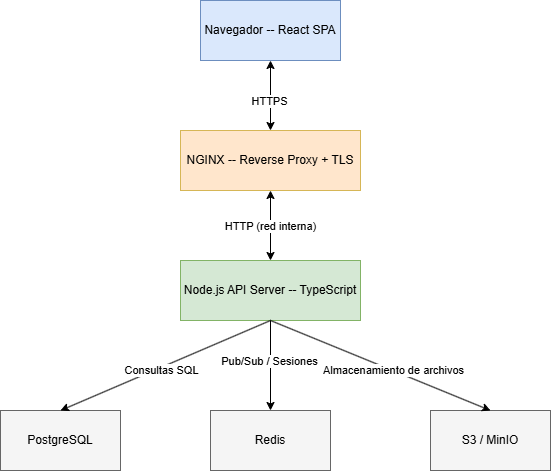
\includegraphics[width=15cm]{Diagrama de Alto Nivel.drawio.png}
        \caption{Diagrama de Arquitectura de Alto Nivel del Sistema Outline}
        \label{fig:placeholder}
    \end{figure}
\end{center}

\chapter*{Priorizar las 8 características de ISO/IEC 25010.}
\addcontentsline{toc}{section}{Priorizar las 8 características de ISO/IEC 25010}



\subsection*{1. Adecuación funcional}
\addcontentsline{toc}{subsection}{1. Adecuación funcional}

 
\subsection*{2. Eficiencia de desempeño}
\addcontentsline{toc}{subsection}{2. Eficiencia de desempeño}


\subsection*{3. Usabilidad}
\addcontentsline{toc}{subsection}{3. Usabilidad}



\subsection*{4. Fiablidad}
\addcontentsline{toc}{subsection}{4. Fiablidad}


\subsection*{5. Seguridad}
\addcontentsline{toc}{subsection}{5. Seguridad}


\subsection*{6. Compatibilidad}
\addcontentsline{toc}{subsection}{6. Compatibilidad}


\subsection*{7. Mantenibilidad}
\addcontentsline{toc}{subsection}{7. Mantenibilidad}


\subsection*{8. Portabilidad}
\addcontentsline{toc}{subsection}{8. Portabilidad}


\newpage

\section*{Calidad en Uso -- Las 2 Características más Relevantes}
\addcontentsline{toc}{section}{Calidad en Uso -- Las 2 Características más Relevantes}



%%%%%%%%%%%%%%%%%%%%%%%%%%%%%%%%%%%%%%%%%%%%%%%%%%%%%%%

\newpage
\chapter*{6 KPIs medibles basados en ISO/IEC 25023}
\addcontentsline{toc}{section}{6 KPIs medibles basados en ISO/IEC 25023}

\subsection*{1. Diponibilidad del servicio}
\addcontentsline{toc}{subsection}{1. Diponibilidad del servicio}
\begin{itemize}
    \item \textbf{Característica ISO 24010: }Fiabilidad -- Disponibilidad \cite{iso25010_2023}
    \item \textbf{Fórmula: } Disponibilidad (\%) = [T\_operativo / (T\_operativo + T\_inactivo)] × 100
    \item \textbf{Umbral: } \geq 99.5\% mensual, lo que equivale a no más de 3.6 horas de caída acumulada en todo el mes
    \item \textbf{Herramienta: } Uptime Kuma instalado en el mismo servidor, revisando el endpoint /api/health.check cada 60 segundos y enviando alertas al canal de Slack del equipo \cite{grafana2024} 
    \item \textbf{Referencia de la métrica: } \cite{iso25023_2016}
\end{itemize}

 



\newpage
\chapter*{Conclusión}
\addcontentsline{toc}{section}{Conclusión}

\printbibliography

\end{document}

